\documentclass[10pt, a4paper]{article}

\usepackage{ctex}
\usepackage{xeCJK}
\usepackage{caption}
\usepackage{geometry}
\geometry{
    left = 0.6in,
    right = 0.6in,
    top = 0.8in,
    bottom = 1.0in
}
\usepackage{amssymb}
\usepackage{amsbsy}
\usepackage{amsmath}
\usepackage{xcolor}
\usepackage{mathrsfs}
\usepackage{graphicx}
\usepackage{pifont}
\usepackage{tikz}
\usepackage{tasks}
\settasks{
    label = \Alph*. ,
    label-width = 16pt
}

\newcommand{\Title}[3]{
    \begin{center}
        \Large \textbf{中国电子学会 #1~年~#2~月 Scratch~#3级考试}
    \end{center}
}
\newcommand{\TimeAndName}[1]{
    \begin{center}
        考试时间:~#1~ 分钟 \qquad\qquad\qquad\qquad 姓名:\underline{\quad\quad\quad\quad}
    \end{center}
}
\pagestyle{empty}
\begin{document}
    \Title{2021}{3}{一}
    
    \TimeAndName{60}
    
    {\noindent\heiti 第一部分、单选题(共 25 题,每题 2 分,共50分.)}

    \begin{enumerate}
        % 1
        % 1
        \item  花花幼儿园有三个班。根据下面三句话,请你猜一猜,哪个班级人数最多?(\qquad)
        
        \ding{172}中班比小班少;\ding{173}中班比大班少;\ding{174}大班比小班多.
        \begin{tasks}(4)
            \task 小班
            \task 中班
            \task 大班
            \task 三个班一样多
        \end{tasks}

        % 2
        \item 下图为有规律排列在一起的9个数字,需要在?处填入正确的数字,以下哪个选项符合规律?(\qquad)
        \begin{tasks}(4)
            \task 15
            \task 20
            \task 25
            \task 30
        \end{tasks}

        \begin{figure}[htbp]
            \centering
            \begin{minipage}[t]{.12\textwidth}
                \centering
                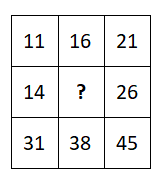
\includegraphics[width=\textwidth]{2.png}
                \caption*{第2题}
            \end{minipage}
            \begin{minipage}[t]{.35\textwidth}
                \centering
                \begin{minipage}[t]{.48\textwidth}
                    \centering
                    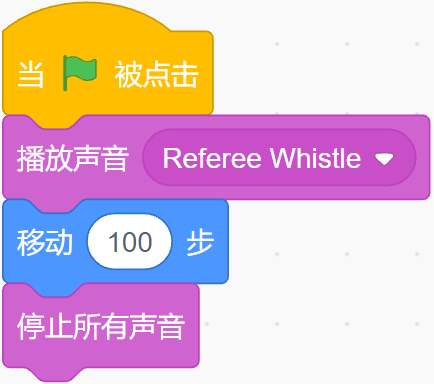
\includegraphics[width=\textwidth]{3-1.png}
                \end{minipage}
                \begin{minipage}[t]{.48\textwidth}
                    \centering
                    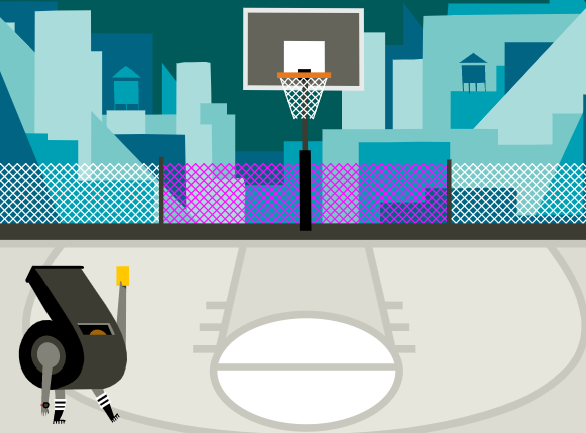
\includegraphics[width=\textwidth]{3-2.png}
                \end{minipage}
                \caption*{第3题}
            \end{minipage}
            \begin{minipage}[t]{.06\textwidth}
                \centering
                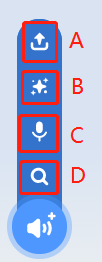
\includegraphics[width=\textwidth]{4.png}
                \caption*{第4题}
            \end{minipage}
            \begin{minipage}[t]{.38\textwidth}
                \centering
                \begin{minipage}[t]{.48\textwidth}
                    \centering
                    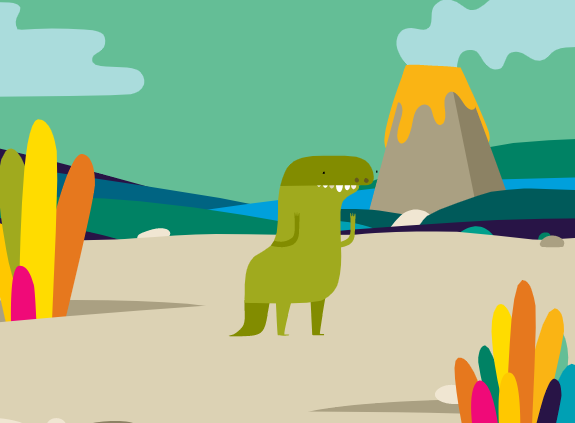
\includegraphics[width=\textwidth]{6-1.png}
                \end{minipage}
                \begin{minipage}[t]{.48\textwidth}
                    \centering
                    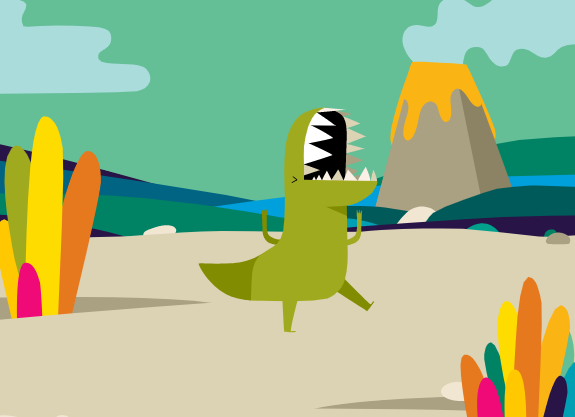
\includegraphics[width=\textwidth]{6-2.png}
                \end{minipage}
                \caption*{第6题}
            \end{minipage}
        \end{figure}

        % 3
        \item 请你根据上面积木块,分析篮球场上哨子角色做了哪些操作?(\qquad)
        \begin{tasks}(2)
            \task 哨子角色仅播放了 Referee whistle声音
            \task 哨子角色播放声音并移动100步后,声音停止
            \task 哨子角色移动200步后声音停止
            \task 哨子角色移动100步后播放声音
        \end{tasks}

        % 4
        % 4
        \item 上面哪个选项可以录制声音?(\qquad)
        \begin{tasks}(4)
            \task A
            \task B
            \task C
            \task D
        \end{tasks}

        % 5
        \item 下图中的小女孩正在进行表演,请你根据下图显示的积木块,判断以下哪个选项是错误的?(\qquad)
        \begin{figure}[htbp]
            \centering
            \begin{minipage}{.12\textwidth}
                \centering
                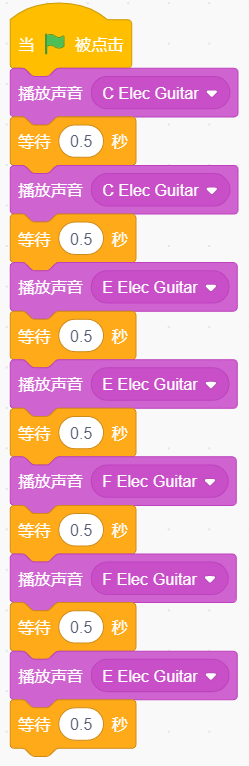
\includegraphics[width=\textwidth]{5-1.png}
            \end{minipage}
            \begin{minipage}{.45\textwidth}
                \begin{tasks}
                    \task 每播放一段声音就等待0.5秒
                    \task 共播放了2次“ C Elec Guitar声音
                    \task 共播放了7次声音
                    \task 共播放了3次“ F Elec guitar”声音
                    \task[*] 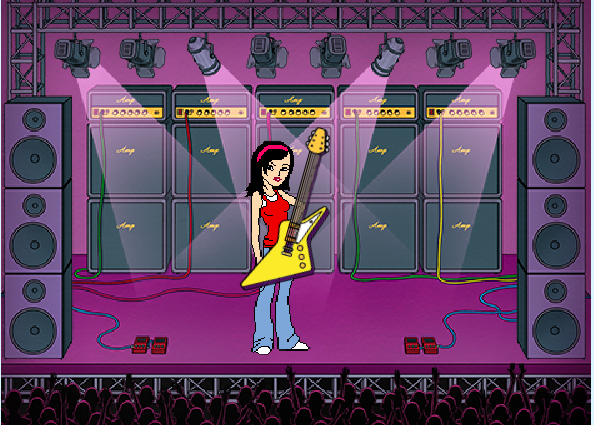
\includegraphics[width=.5\textwidth]{5-2.png}
                \end{tasks}
            \end{minipage}
        \end{figure}

        % 6
        \item 上图为恐龙角色的初始状态,当恐龙角色遇到危险时就会张大嘴巴(变为dinosaur4-d造型),以下哪个程序可以让恐龙角色张大嘴巴?(\qquad)
        \begin{tasks}(4)
            \task 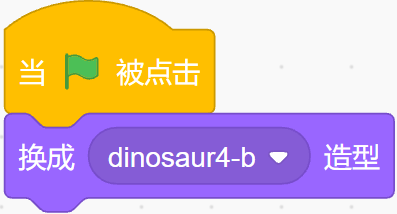
\includegraphics[width=.15\textwidth]{6a.png}
            \task 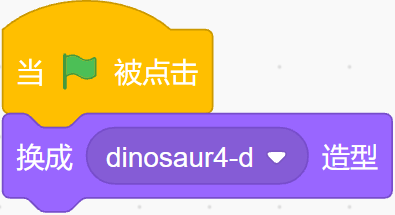
\includegraphics[width=.15\textwidth]{6b.png}
            \task 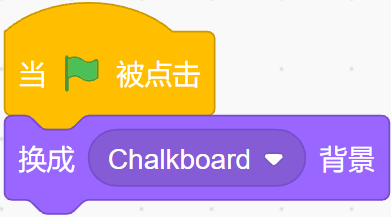
\includegraphics[width=.15\textwidth]{6c.png}
            \task 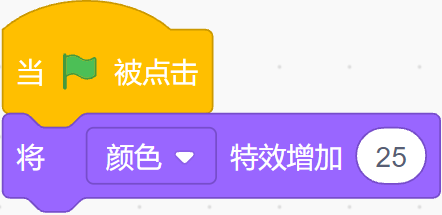
\includegraphics[width=.17\textwidth]{6d.png}
        \end{tasks}

        \newpage
        % 7
        \item 小明边听音乐边写作业,妈妈让他把音乐声减小,于是小明决定写一个程序,控制音箱声音的大小,下面哪个积木可以帮助小明减小音箱的音量?(\qquad)
        \begin{tasks}(4)
            \task 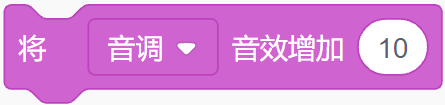
\includegraphics[width=.18\textwidth]{7a.png}
            \task 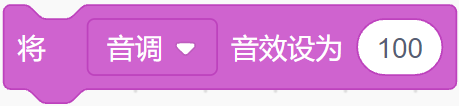
\includegraphics[width=.18\textwidth]{7b.png}
            \task 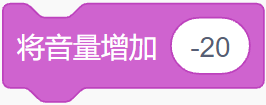
\includegraphics[width=.12\textwidth]{7c.png}
            \task 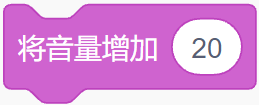
\includegraphics[width=.12\textwidth]{7d.png}
        \end{tasks}
           
        % 8
        \item 放学之后,小明从学校回到家中,学校和家的背景如上图依次为School、Family,执行以下哪个程序可以让小明从School背景变为Family背景?(\qquad)
        \begin{tasks}(4)
            \task 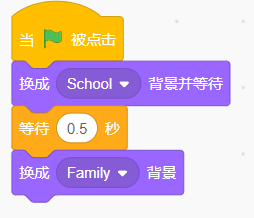
\includegraphics[width=.15\textwidth]{8a.png}
            \task 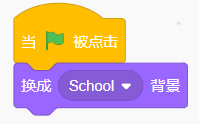
\includegraphics[width=.15\textwidth]{8b.png}
            \task 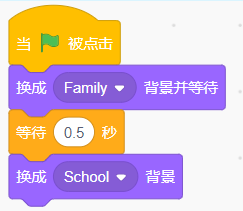
\includegraphics[width=.15\textwidth]{8c.png}
            \task 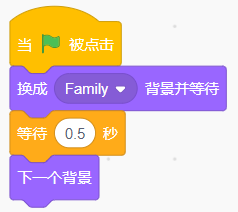
\includegraphics[width=.15\textwidth]{8d.png}
        \end{tasks}

        \begin{figure}[htbp]
            \centering
            \begin{minipage}[t]{.18\textwidth}
                \centering
                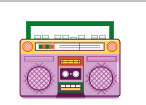
\includegraphics[width=\textwidth]{7.png}
                \caption*{第7题}
            \end{minipage}
            \begin{minipage}[t]{.07\textwidth}
                \centering
                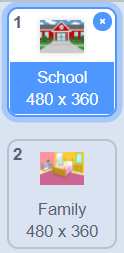
\includegraphics[width=\textwidth]{8.png}
                \caption*{第8题}
            \end{minipage}
            \begin{minipage}[t]{.18\textwidth}
                \centering
                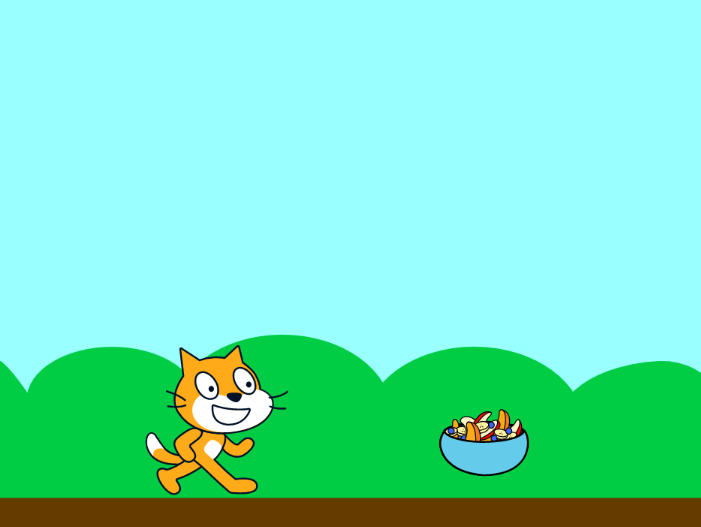
\includegraphics[width=\textwidth]{9.png}
                \caption*{第9题}
            \end{minipage}
            \begin{minipage}[t]{.18\textwidth}
                \centering
                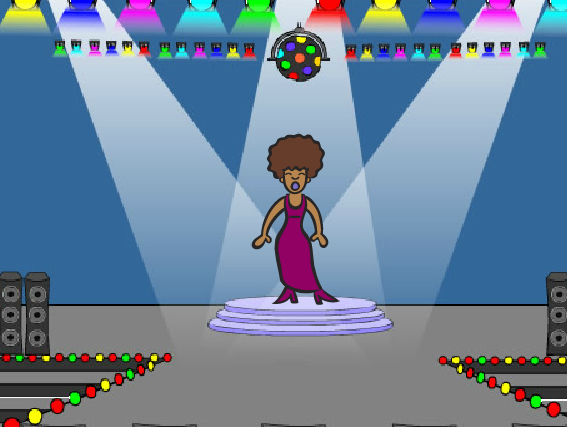
\includegraphics[width=\textwidth]{10.png}
                \caption*{第10题}
            \end{minipage}
            \begin{minipage}[t]{.3\textwidth}
                \centering
                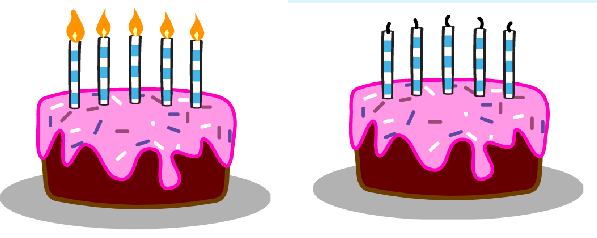
\includegraphics[width=\textwidth]{11.png}
                \caption*{第11题}
            \end{minipage}
        \end{figure}

        % 9
        \item 如上图,小猫右边,距离200步的位置上有一碗水果,只执行一次下面哪个程序可以让小猫吃到水果?(\qquad)
        \begin{tasks}(4)
            \task 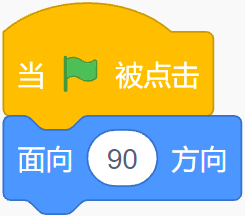
\includegraphics[width=.12\textwidth]{9a.png}
            \task 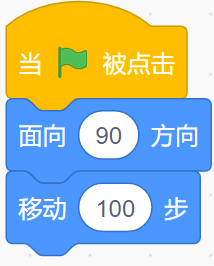
\includegraphics[width=.1\textwidth]{9b.png}
            \task 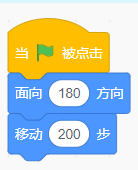
\includegraphics[width=.1\textwidth]{9c.png}
            \task 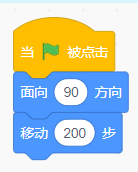
\includegraphics[width=.1\textwidth]{9d.png}
        \end{tasks}

       % 10
       \item 如上图所示,随着舞台灯光的变化,以下哪个程序可以实现女孩角色播放Dance Magic音乐,然后颜色特效增加25?(\qquad)
        \begin{tasks}(4)
            \task 
\includegraphics[width=.15\textwidth]{10a.png}
            \task 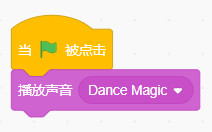
\includegraphics[width=.15\textwidth]{10b.png}
            \task 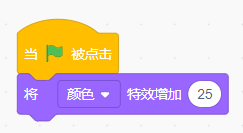
\includegraphics[width=.15\textwidth]{10c.png}
            \task 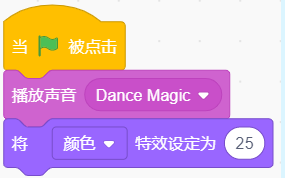
\includegraphics[width=.15\textwidth]{10d.png}
        \end{tasks}

        % 11
        \item 小明要过生日啦,如上图所示蛋糕的2个造型依次为cake-a、cake-b,现在默认的造型是cake-a蜡烛为点亮状态,以下哪个程序可以帮助小明熄灭蛋糕上的蜡烛?(\qquad)
        \begin{tasks}(4)
            \task 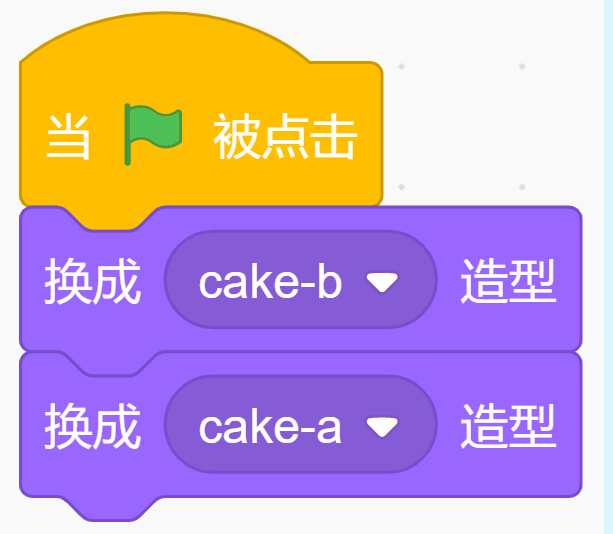
\includegraphics[width=.12\textwidth]{11a.png}
            \task 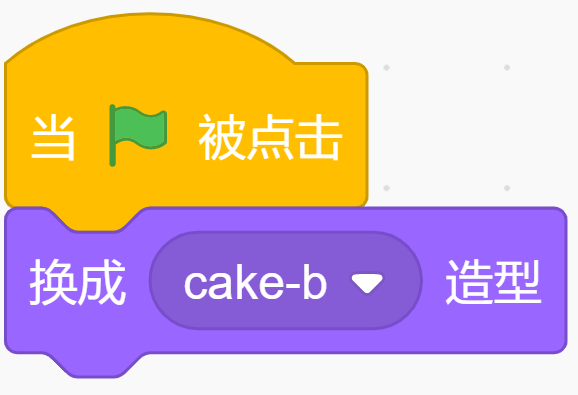
\includegraphics[width=.15\textwidth]{11b.png}
            \task 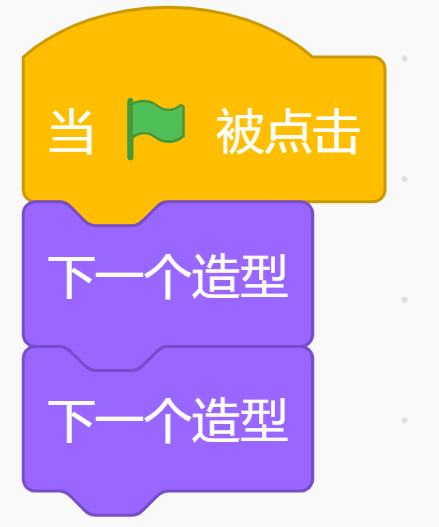
\includegraphics[width=.09\textwidth]{11c.png}
            \task 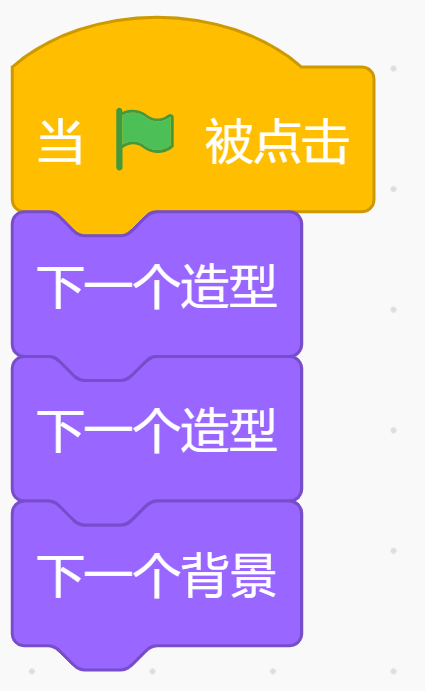
\includegraphics[width=.07\textwidth]{11d.png}
        \end{tasks}
        
        % 12
        \item 如下图,炎炎夏日,小明想要吃西瓜消暑,以下哪个程序可以让小明得到西瓜?(\qquad)
        
        \begin{minipage}{.06\textwidth}
            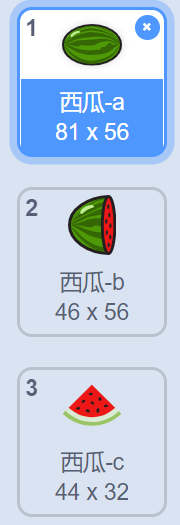
\includegraphics[width=\textwidth]{12.png}
        \end{minipage}
        \begin{minipage}{.8\textwidth}
            \begin{tasks}(4)
                \task 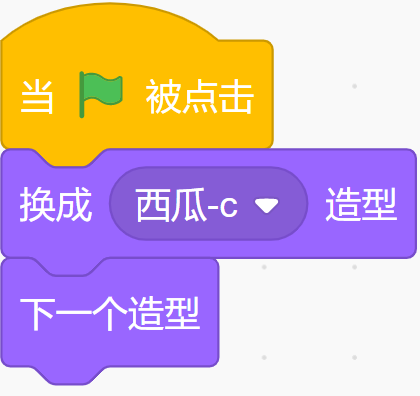
\includegraphics[width=.15\textwidth]{12a.png}
                \task 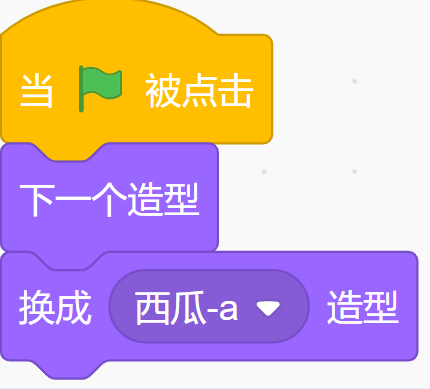
\includegraphics[width=.15\textwidth]{12b.png}
                \task 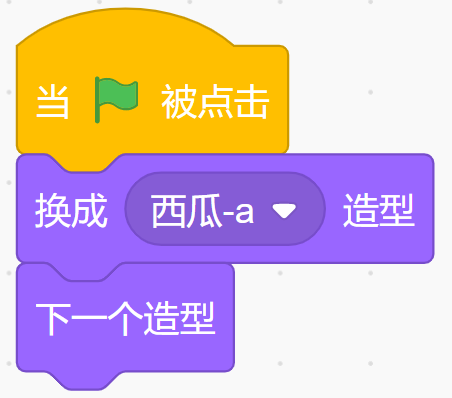
\includegraphics[width=.15\textwidth]{12c.png}
                \task 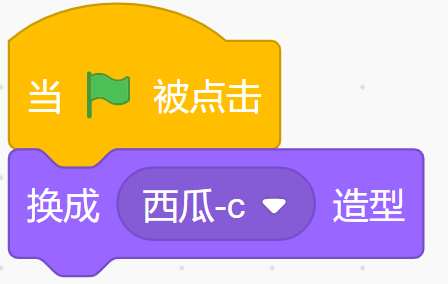
\includegraphics[width=.18\textwidth]{12d.png}
            \end{tasks}
        \end{minipage}

        \newpage
        % 13
        \item 一块豆腐平放着按照下图所示的方式切4刀,我们会得到几块豆腐?(\qquad)
        \begin{tasks}(4)
            \task 4
            \task 6
            \task 8
            \task 9
        \end{tasks}

        % 14
        \item 执行以下程序后,关于小青蛙的描述正确的是?(\qquad)
        \begin{tasks}(2)
            \task 小青蛙叫一声“呱”之后,向前走50步
            \task 小青蛙一边叫一声“呱”一边向前走50步
            \task 小青蛙先向前走50步之后,再叫一声“呱”
            \task 小青蛙原地不动
        \end{tasks}

        \begin{figure}[htbp]
            \centering
            \begin{minipage}[t]{.16\textwidth}
                \centering
                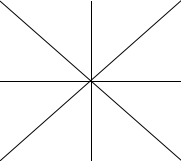
\includegraphics[width=\textwidth]{13.png}
                \caption*{第13题}
            \end{minipage}
            \begin{minipage}[t]{.38\textwidth}
                \centering
                \begin{minipage}[t]{.4\textwidth}
                    \centering
                    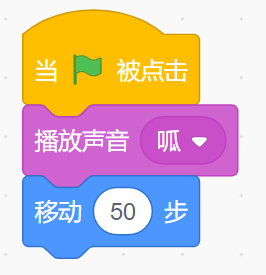
\includegraphics[width=\textwidth]{14-1.png}
                \end{minipage}
                \begin{minipage}[t]{.58\textwidth}
                    \centering
                    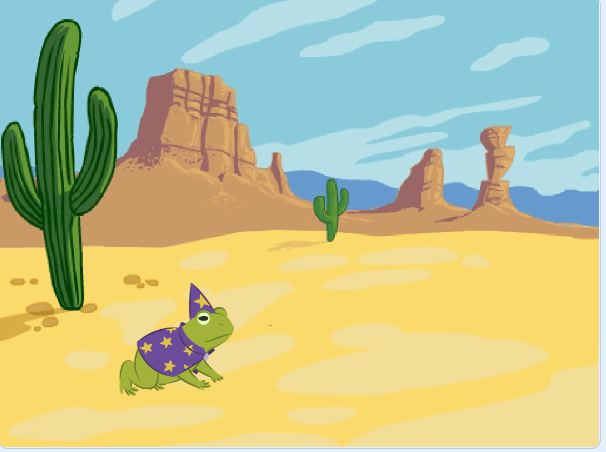
\includegraphics[width=\textwidth]{14-2.png}
                \end{minipage}
                \caption*{第14题}
            \end{minipage}
            \begin{minipage}[t]{.23\textwidth}
                \centering
                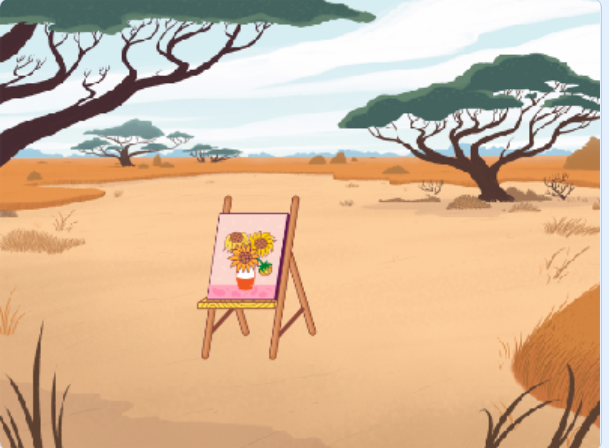
\includegraphics[width=\textwidth]{15.png}
                \caption*{第15题}
            \end{minipage}
        \end{figure}
    
        % 15
        \item  画架的造型如下图所示,小丽拿着画架去室外画画时,以下哪个积木块运行一次就可以看到小丽最终画的效果(造型Easel-c)?(\qquad)
        \begin{tasks}(4)
            \task 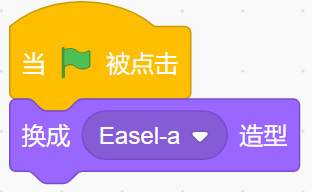
\includegraphics[width=.15\textwidth]{15a.png}
            \task 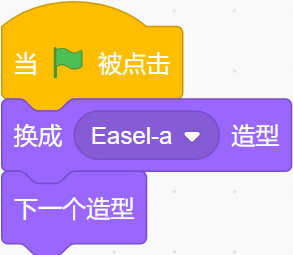
\includegraphics[width=.11\textwidth]{15b.png}
            \task 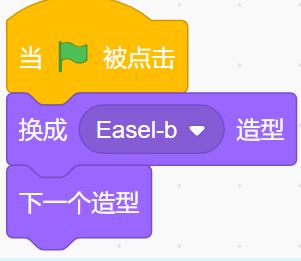
\includegraphics[width=.11\textwidth]{15c.png}
            \task 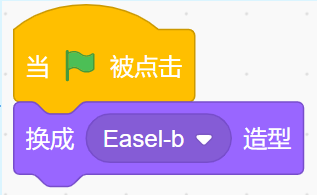
\includegraphics[width=.15\textwidth]{15d.png}
        \end{tasks}
        
        % 16
        \item 点击下面哪个按钮可以停止程序运行?(\qquad)
        \begin{tasks}(4)
            \task \includegraphics[width=.05\textwidth]{16a.png}
            \task \includegraphics[width=.05\textwidth]{16b.png}
            \task \includegraphics[width=.05\textwidth]{16c.png}
            \task \includegraphics[width=.05\textwidth]{16d.png}
        \end{tasks}

        % 17
        \item  炎热的夏天到了,小刚想在自己的scratch作品中加入泳池的背景,以下哪个背景符合小刚的要求?(\qquad)
        \begin{tasks}(4)
            \task \includegraphics[width=.18\textwidth]{17a.png}
            \task \includegraphics[width=.18\textwidth]{17b.png}
            \task \includegraphics[width=.18\textwidth]{17c.png}
            \task \includegraphics[width=.18\textwidth]{17d.png}
        \end{tasks}

        % 18
        \item 根据下面三幅图片的阴影变化规律,第四幅图片为以下哪个选项?(\qquad)
        
        \begin{figure}[htbp]
            \centering
            \includegraphics[width=.5\textwidth]{18.png}
        \end{figure}
        \begin{tasks}(4)
            \task \includegraphics[width=.15\textwidth]{18a.png}
            \task \includegraphics[width=.15\textwidth]{18b.png}
            \task \includegraphics[width=.15\textwidth]{18c.png}
            \task \includegraphics[width=.15\textwidth]{18d.png}
        \end{tasks}

        % 19
        \item  角色的造型(从上到下分别为a,b,c,d)和初始状态如下图所示,执行以下程序后,哪个选项描述不正确?(\qquad)
        \begin{tasks}(2)
            \task 角色一共移动30步
            \task 角色切换了四次造型
            \task 积木块运行过程中没有切换背景
            \task 角色最后的造型为avery walking-d
        \end{tasks}

        \begin{figure}[htbp]
            \centering
            \begin{minipage}[t]{.58\textwidth}
                \centering
                \begin{minipage}[t]{.13\textwidth}
                    \centering
                    \includegraphics[width=\textwidth]{19-1.png}
                \end{minipage}
                \begin{minipage}[t]{.2\textwidth}
                    \centering
                    \includegraphics[width=\textwidth]{19-2.png}
                \end{minipage}
                \begin{minipage}[t]{.48\textwidth}
                    \centering
                    \includegraphics[width=\textwidth]{19-3.png}
                \end{minipage}
                \caption*{第19题}
            \end{minipage}
            \begin{minipage}[t]{.1\textwidth}
                \centering
                \includegraphics[width=\textwidth]{21.png}
                \caption*{第21题}
            \end{minipage}
            \begin{minipage}[t]{.3\textwidth}
                \centering
                \begin{minipage}[t]{.4\textwidth}
                    \centering
                    \includegraphics[width=\textwidth]{22-1.png}
                \end{minipage}
                \begin{minipage}[t]{.58\textwidth}
                    \centering
                    \includegraphics[width=\textwidth]{22-2.png}
                \end{minipage}
                \caption*{第22题}
            \end{minipage}
        \end{figure}

        % 20
        \item  以下哪个选项是左右平衡音效中音效的最大值?(\qquad)
        \begin{tasks}(4)
            \task 100
            \task 150
            \task 50
            \task 25
        \end{tasks}

        % 21
        \item 如上图所示青蛙有三个造型,青蛙只有变成Frog 2-c时候才可以吃到虫子,执行下面哪个程序可以让青蛙从Frog 2-a变为Frog 2-c?(\qquad)
        \begin{tasks}(4)
            \task \includegraphics[width=.1\textwidth]{21a.png}
            \task \includegraphics[width=.13\textwidth]{21b.png}
            \task \includegraphics[width=.13\textwidth]{21c.png}
            \task \includegraphics[width=.13\textwidth]{21d.png}
        \end{tasks}

        % 22
        \item 小猫初始位置如上图所示,点击绿旗后,小猫面向的方向为多少?(\qquad)
        \begin{tasks}(4)
            \task 面向45方向
            \task 面向90方向
            \task 面向75方向
            \task 面向0方向
        \end{tasks}

        % 23
        \item  下面哪个程序可以让小北极熊沿着箭头走到大北极熊的身边?(\qquad)
        
        \begin{minipage}{.2\textwidth}
            \includegraphics[width=\textwidth]{23.png}
        \end{minipage}
        \begin{minipage}{.7\textwidth}
            \begin{tasks}(4)
                \task \includegraphics[width=.12\textwidth]{23a.png}
                \task \includegraphics[width=.12\textwidth]{23b.png}
                \task \includegraphics[width=.18\textwidth]{23c.png}
                \task \includegraphics[width=.18\textwidth]{23d.png}
            \end{tasks}
        \end{minipage}

        % 24
        \item 如下图,下面哪个选项可以修改小猫的大小?(\qquad)
        
        \begin{minipage}{.15\textwidth}
            \includegraphics[width=\textwidth]{24.png}
        \end{minipage}
        \begin{minipage}{.7\textwidth}
            \begin{tasks}(4)
                \task \ding{172}
                \task \ding{173}
                \task \ding{174}
                \task \ding{175}
            \end{tasks}
        \end{minipage}
        
        % 25
        \item 如上图,演唱会时架子鼓的声音太小了,以下哪个程序运行一次可以将架子鼓的音量设置100\%?(\qquad)
        
        \begin{minipage}{.15\textwidth}
            \includegraphics[width=\textwidth]{25.png}
        \end{minipage}
        \begin{minipage}{.75\textwidth}
            \begin{tasks}(4)
                \task \includegraphics[width=.18\textwidth]{25a.png}
                \task \includegraphics[width=.16\textwidth]{25b.png}
                \task \includegraphics[width=.18\textwidth]{25c.png}
                \task \includegraphics[width=.16\textwidth]{25d.png}
            \end{tasks}
        \end{minipage}
    \end{enumerate}

    \newpage
    {\noindent\heiti 第二部分、判断题(共 10 题,每题 2 分,共20分.)}
    \begin{enumerate}
        \setcounter{enumi}{25}
        % 26
        \item 根据下列三个算式可知,\tikz\draw (0,0) rectangle (8pt,8pt); \quad \tikz\draw (0,0) circle (4pt); \quad \tikz\draw (0,0) -- (0.4,0) -- (0.2,0.346) -- cycle; 的值分别为1,2,3.(\qquad)

        \begin{figure}[htbp]
            \centering
            \begin{minipage}[t]{.18\textwidth}
                \centering
                \includegraphics[width=\textwidth]{26.png}
                \caption*{第26题}
            \end{minipage}
            \begin{minipage}[t]{.48\textwidth}
                \centering
                \begin{minipage}[t]{.4\textwidth}
                    \centering
                    \includegraphics[width=\textwidth]{27-1.png}
                \end{minipage}
                \begin{minipage}[t]{.25\textwidth}
                    \centering
                    \includegraphics[width=\textwidth]{27-2.png}
                \end{minipage}
                \caption*{第27题}
            \end{minipage}
            \begin{minipage}[t]{.3\textwidth}
                \centering
                \includegraphics[width=0.9\textwidth]{28.png}
                \caption*{第28题}
            \end{minipage}
        \end{figure}

        %27
        \item 上面程序能实现等待声音播放完成后再进行造型的切换.(\qquad)
        
        %28
        \item 修改上图红框内容,可以改变声音的名字.(\qquad)
  
        %29
        \item 下图所示,图中的红框位置可以实现背景水平翻.(\qquad)
        
        %30
        \item 使用如图\includegraphics[width=.08\textwidth]{30.png}所示的积木可以实现在背景之间按顺序切换,最后一个背景之后又会切换到第一个背景,依次反复.(\qquad)
        
        \begin{figure}[htbp]
            \centering
            \begin{minipage}[t]{.25\textwidth}
                \centering
                \includegraphics[width=\textwidth]{29.png}
                \caption*{第29题}
            \end{minipage}
            \begin{minipage}[t]{.18\textwidth}
                \centering
                \begin{minipage}[t]{.35\textwidth}
                    \centering
                    \includegraphics[width=\textwidth]{31-1.png}
                \end{minipage}
                \begin{minipage}[t]{.55\textwidth}
                    \centering
                    \includegraphics[width=\textwidth]{31-2.png}
                \end{minipage}
                \caption*{第31题}
            \end{minipage}
            \begin{minipage}[t]{.48\textwidth}
                \centering
                \begin{minipage}[t]{.48\textwidth}
                    \centering
                    \includegraphics[width=\textwidth]{32-1.png}
                \end{minipage}
                \begin{minipage}[t]{.4\textwidth}
                    \centering
                    \includegraphics[width=\textwidth]{32-2.png}
                \end{minipage}
                \caption*{第32题}
            \end{minipage}
        \end{figure}

        %31
        \item 裙子的造型如上图所示,执行上面程序后,可以看到裙子按照造型dress-a,dress-b,dress-c的顺序变化.(\qquad)
        
        %32
        \item 上面程序实现女孩角色移动150步后立即播放音乐.(\qquad)
        
        %33
        \item 下面程序可以实现火箭角色,移动100步后大小减少20.(\qquad)
        
        %34
        \item 两个角色的程序如下图所示,点击绿旗后,按下空格键,将停止正在播放的所有声音.(\qquad)
        
        \begin{figure}[htbp]
            \centering
            \begin{minipage}[t]{.25\textwidth}
                \centering
                \begin{minipage}[t]{.38\textwidth}
                    \centering
                    \includegraphics[width=\textwidth]{33-1.png}
                \end{minipage}
                \begin{minipage}[t]{.5\textwidth}
                    \centering
                    \includegraphics[width=\textwidth]{33-2.png}
                \end{minipage}
                \caption*{第33题}
            \end{minipage}
            \begin{minipage}[t]{.28\textwidth}
                \centering
                \begin{minipage}[t]{.48\textwidth}
                    \centering
                    \includegraphics[width=\textwidth]{34-1.png}
                \end{minipage}
                \begin{minipage}[t]{.4\textwidth}
                    \centering
                    \includegraphics[width=\textwidth]{34-2.png}
                \end{minipage}
                \caption*{第34题}
            \end{minipage}
        \end{figure}
        
        %35
        \item 可以对声音进行快一点、慢一点、响一点、轻一点的操作,但是不能进行修剪的操作.(\qquad)
    \end{enumerate}

    \newpage
    {\noindent\heiti 第三部分、编程题(共 2 题,共30分.)}
    \begin{enumerate}
        \setcounter{enumi}{35}
        
        % 36
        \item 小镇一日游:
        
        1. 准备工作
        \begin{tasks}[label = (\arabic*)]
            \task 选择背景Colorful City、School、Urban以及Night City With Street;
            \task 去掉小猫角色;
            \task 选择City Bus汽车角色,添加Car Horn声音.
        \end{tasks}
        2. 功能实现
        \begin{tasks}[label = (\arabic*)]
            \task 初始的背景为Colorful City,汽车的初始位置在屏幕右下角,面向右面;
            \task 点击绿旗,汽车角色向左移动50步后从City Bus-a造型切换到City Bus-b造型,之后播放Car Hom声音,等待两秒后进入School背景;
            \task 进入School背景后汽车向左移动50步,播放Car Hom声,等待两秒后进入Urban背景;
            \task 进入Urban背景后汽车向左移动50步,播放Car Hom声音,等待两秒后进入背景Night City With Street;
            \task 进入背景Night City With Street后汽车向左移动50步,播放Car Horn声音。
        \end{tasks}
        \begin{figure}[htbp]
            \begin{minipage}[t]{.48\textwidth}
                \centering
                \includegraphics[width=.6\textwidth]{36.png}
                \caption*{第 36 题}
            \end{minipage}
            \begin{minipage}[t]{.48\textwidth}
                \centering
                \includegraphics[width=.6\textwidth]{37.png}
                \caption*{第 37 题}
            \end{minipage}
        \end{figure}
                

        %37
        \item 棒球运动会:

        1. 准备工作
        \begin{tasks}[label = (\arabic*)]
            \task 选择背景Baseball1;
            \task 去掉小猫角色;
            \task 添加角色Batter、添加声音Basketball Bounce;
            \task 球角色Baseball。
        \end{tasks}
        2. 功能实现
        \begin{tasks}[label = (\arabic*)]
            \task 初始的背景为Baseball 1;
            \task 设置人物角色Batter和棒球角色Basebal的初始位置如下图所示,人物角色Batter和棒球Baseball1在同一水平线上,它们相距65步;
            \task 点击绿旗,设置人物角色造型为batter-a,等待0.5秒后,人物角色Batter向左移动65步,之后人物角色Batter的造型切换成batter-b,再次等待0.5秒,人物角色Batter的造
            型切换成batter-C;
            \task 在人物角色Batter的造型切换成batter-c的时候播放声音Basketball Bounce,并说“我打到了”2秒.
        \end{tasks}
    \end{enumerate}
\end{document}